\begin{frame}
    \frametitle{Наборы данных для исследования}
    Для исследования качества решений и временной сложности алгоритма были созданы следующие наборы данных:
    \begin{enumerate}
        \item Набор данных с известным оптимумом.
        % \begin{itemize}
        %     \item 2000; 5000; 10000; 20000; 30000; 40000; 50000; 75000; 100000 работ
        % \end{itemize}
        \item Набор данных, основанных на слоистых данных.
        % \begin{itemize}
        %     \item 
        % \end{itemize}
        \item Набор данных для построения расписания на неоднородных процессорах.
        % \begin{itemize}
        %     \item 
        % \end{itemize}
    \end{enumerate}
\end{frame}

\begin{frame}
    \frametitle{Точность полученного расписания. CR}
    \begin{figure}
        \begin{subfigure}{0.49\textwidth}
            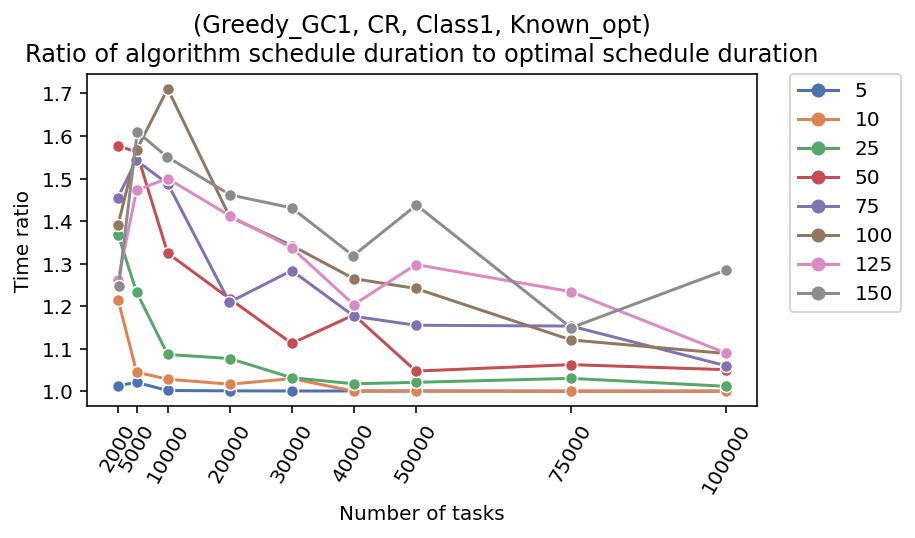
\includegraphics[width=\textwidth]{imgs/ideal_1/CR/gr_amalgamated.png}
            \caption{Жадный алгоритм с выбором по числу потомков}
        \end{subfigure}
        \begin{subfigure}{0.49\textwidth}
            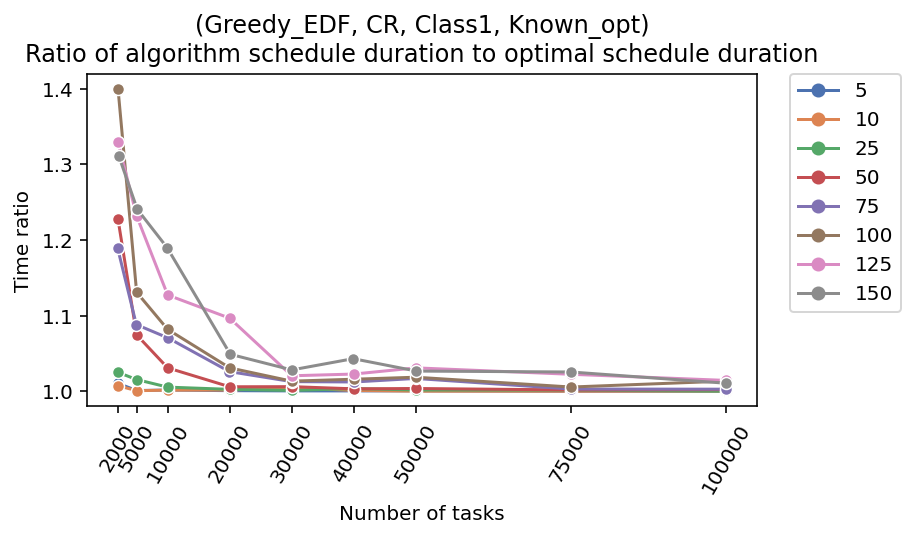
\includegraphics[width=\textwidth]{imgs/ideal_1/CR_EDF/gr_amalgamated.png}
            \caption{Жадный алгоритм с фиктивными директивными сроками}
        \end{subfigure}
        \caption{Качество решений алгоритмов на данных с известным оптимумом,\\ постановка с дополнительным ограничением на межпроцессорные передачи}
    \end{figure}
\end{frame}

\begin{frame}
    \frametitle{Точность полученного расписания. NO}
    \begin{figure}
        \begin{subfigure}{0.49\textwidth}
            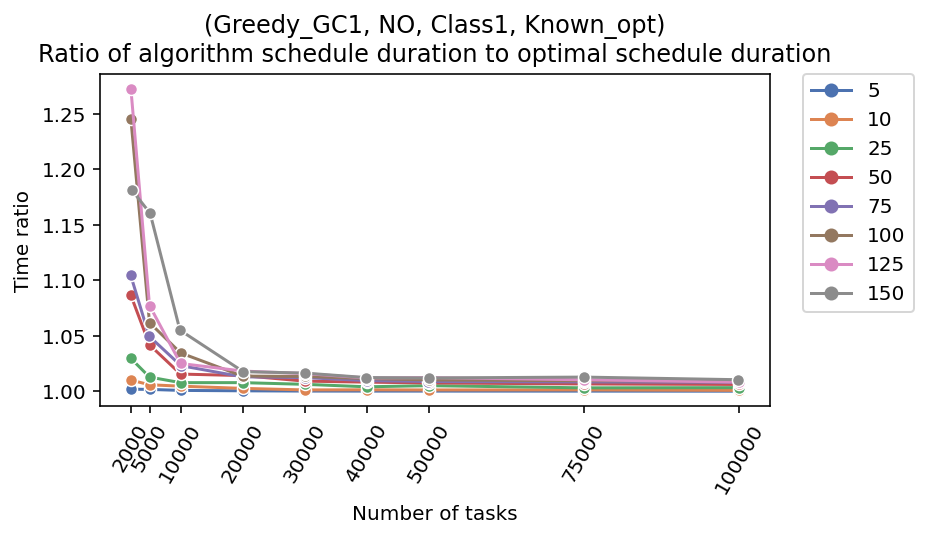
\includegraphics[width=\textwidth]{imgs/ideal_1/NO/gr_amalgamated.png}
            \caption{Жадный алгоритм с выбором по числу потомков}
        \end{subfigure}
        \begin{subfigure}{0.49\textwidth}
            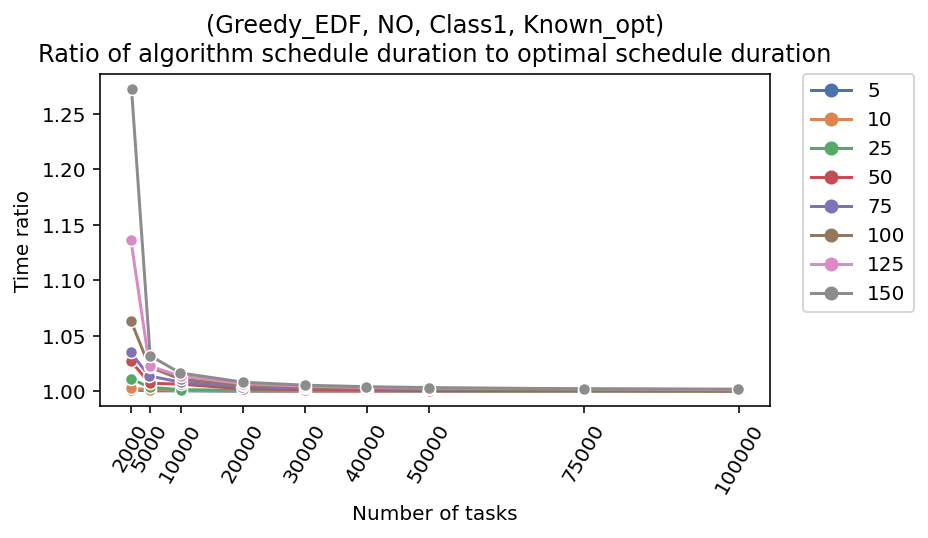
\includegraphics[width=\textwidth]{imgs/ideal_1/NO_EDF/gr_amalgamated.png}
            \caption{Жадный алгоритм с фиктивными директивными сроками}
        \end{subfigure}
        \caption{Качество решений алгоритмов на данных с известным оптимумом,\\ постановка без дополнительных ограничений}
    \end{figure}
\end{frame}

